%%%%%%%%%%%%%%%%%%%%%%%%%%%%%%%%%_TEMPLATE_PACKAGES_%%%%%%%%%%%%%%%%%%%%%%%%%%%%%%%%%
\documentclass[
	a4paper,
	pagesize,
	pdftex,
	12pt,
	% twoside,    % + BCOR darunter: für doppelseitigen Druck aktivieren, sonst beide deaktivieren
	% BCOR=5mm,   % Dicke der Bindung berücksichtigen (Copyshop fragen, wie viel das ist)
	ngerman,
	fleqn,
	final,
	]{scrartcl}
    
% PACKAGES FOR THE INSTITUTSVORLAGE
\usepackage[utf8]{inputenc}
\usepackage[english]{babel}
\usepackage{listofitems} % for \readlist to create arrays
\usepackage[unicode=true]{hyperref} % label, references, websites and crosslinks in PDF
\usepackage{setspace} % für Elemente der Titelseite
\usepackage{tikz} % für Elemente der Titelseite
\usepackage{tabularx} % für Elemente der Titelseite
\usepackage[draft=false,babel,tracking=true,kerning=true,spacing=true]{microtype} % optischer Randausgleich
% PACKAGES FOR USING THIS PREBUILD STUCTURE
\usepackage{csquotes}   % better quote style for biblatex
\usepackage{graphicx}
%%%%%%%%%%%%%%%%%%%%%%%%%%%%%%%%%_YOUR_PACKAGES_%%%%%%%%%%%%%%%%%%%%%%%%%%%%%%%%%
% UTILITY PACKAGES
% \usepackage{cite}
\usepackage[sorting=none]{biblatex}
\addbibresource{library/citations.bib}
\usepackage{comment} % enables block comments via \begin{comment} ... \end{comment} environment
\usepackage{amsthm} % for definitions, lemmas, etc. - also for defining your own stuff, eg below:
    %\theoremstyle{definition}  % defines a new theorem called definition
    %\newtheorem{definition}{Definition}[section]   % definition setup and call
\usepackage{todonotes}
% IMAGE PACKAGES
\usepackage{wrapfig}    % create figures with wrapped text around it
\usepackage{caption}    % better captions for figures
\usepackage{subcaption} % captions for subfigures
% PRESENTATION PACKAGES
\usepackage{booktabs} % for professional tables
\usepackage{longtable} % for tables over multiple pages
\usepackage{pdflscape} % enables landscape mode for multiple pages in PDF (with longtable)
\usepackage{afterpage} % clears current page by flushing all floats
\usepackage{amssymb}
\usepackage{mathtools}
\usepackage{amsmath} % for aligned
\usepackage{listofitems} % for \readlist to create arrays
\usetikzlibrary{arrows.meta} % for arrow size
\usepackage[outline]{contour} % glow around text
\usepackage{graphicx}
\usetikzlibrary{calc}
\usepackage{caption}
\newtheorem{definition}{Definition}


\graphicspath{ {./images/} }
\DeclareUnicodeCharacter{0308}{HERE!HERE!}

% STYLES
\tikzset{
  >=latex, % for default LaTeX arrow head
  node/.style={thick,circle,draw=myblue,minimum size=22,inner sep=0.5,outer sep=0.6},
  node in/.style={node,green!20!black,draw=mygreen!30!black,fill=mygreen!25},
  node hidden/.style={node,blue!20!black,draw=myblue!30!black,fill=myblue!20},
  node convol/.style={node,orange!20!black,draw=myorange!30!black,fill=myorange!20},
  node out/.style={node,red!20!black,draw=myred!30!black,fill=myred!20},
  connect/.style={thick,mydarkblue}, %,line cap=round
  connect arrow/.style={-{Latex[length=4,width=3.5]},thick,mydarkblue,shorten <=0.5,shorten >=1},
  node 1/.style={node in}, % node styles, numbered for easy mapping with \nstyle
  node 2/.style={node hidden},
  node 3/.style={node out}
}
\def\nstyle{int(\lay<\Nnodlen?min(2,\lay):3)} % map layer number onto 1, 2, or 3

% COLORS
\usepackage{xcolor}
\colorlet{myred}{red!80!black}
\colorlet{myblue}{blue!80!black}
\colorlet{mygreen}{green!60!black}
\colorlet{myorange}{orange!70!red!60!black}
\colorlet{mydarkred}{red!30!black}
\colorlet{mydarkblue}{blue!40!black}
\colorlet{mydarkgreen}{green!30!black}
%%%%%%%%%%%%%%%%%%%%%%%%%%%%%%%%%%%_TITLE_PAGE_%%%%%%%%%%%%%%%%%%%%%%%%%%%%%%%%%%%
\begin{document}

% Beispielhafte Nutzung der Vorlage für die Titelseite (bitte anpassen):
% LaTeX-Vorlage für die Titelseite und Selbständigkeitserklärung einer Abschlussarbeit
% basierend auf der vorigen Institutsvorlage des Instituts für Informatik
% sowie der Vorlage für Promotionsarbeiten.
%%%%%%%%%%%%%%%%%%%%%%%%%%%%%%%%%%%%%%%%%%%%%%%%%%%%%%%%%%%%%%%%%%%%%%%%%%%%%%%%%%%%
% CHANGELOG
% 2014-06-12 Dennis Schneider <dschneid@informatik.hu-berlin.de> (Erweiterung)
% 2023-02-28 Anna Göing <goeingan@informatik.hu-berlin.de> (Strukturhilfe + Packageupdate) 
% 2023-07-14 Florian Willich <florian.willich@informatik.hu-berlin.de> (Formal Revision, Abstract, Package Revision)
%%%%%%%%%%%%%%%%%%%%%%%%%%%%%%%%%%%%%%%%%%%%%%%%%%%%%%%%%%%%%%%%%%%%%%%%%%%%%%%%%%%%
% gepunktete Linie unter Objekt:
\newcommand{\TitelPunkte}[1]{%
  \tikz[baseline=(todotted.base)]{
    \node[inner sep=1pt,outer sep=0pt] (todotted) {#1};
    \draw[dotted] (todotted.south west) -- (todotted.south east);
  }%
}%
% gepunktete Linie mit gegebener Länge:
\newcommand{\TitelPunktLinie}[1]{\TitelPunkte{\makebox[#1][l]{}}}
\makeatletter
%
\newcommand*{\@titelTitel}{Titel der Arbeit}
\newcommand{\titel}[1]{\renewcommand*{\@titelTitel}{#1}} % Titel der Arbeit
\newcommand*{\@titelArbeit}{Arbeitstyp}
\newcommand{\typ}[1]{\renewcommand*{\@titelArbeit}{#1}} % Typ der Arbeit
\newcommand*{\@titelGrad}{akademischer Grad}
\newcommand{\grad}[1]{\renewcommand*{\@titelGrad}{#1}} % Akademischer Grad
\newcommand*{\@titelAutor}{Autor}
\newcommand{\autor}[1]{\renewcommand*{\@titelAutor}{#1}} % Autor der Arbeit
\newcommand*{\@titelGeburtsdatum}{\TitelPunktLinie{2cm}}
\newcommand{\gebdatum}[1]{\renewcommand*{\@titelGeburtsdatum}{#1}} % Geburtsdatum des Autors
\newcommand*{\@titelGeburtsort}{\TitelPunktLinie{5cm}}
\newcommand{\gebort}[1]{\renewcommand*{\@titelGeburtsort}{#1}} % Geburtsort des Autors
\newcommand*{\@titelGutachterA}{\TitelPunktLinie{5cm}}
\newcommand*{\@titelGutachterB}{\TitelPunktLinie{5cm}}
\newcommand*{\@titelAdvisor}{\TitelPunktLinie{5cm}}
\newcommand{\advisor}[1]{\renewcommand*{\@titelAdvisor}{#1}}
\newcommand{\gutachter}[2]{\renewcommand*{\@titelGutachterA}{#1}\renewcommand*{\@titelGutachterB}{#2}} % Erst- und Zweitgutachter
\newcommand*{\@titelEinreichungsdatum}{\TitelPunktLinie{3cm}} % Datum der Einreichung, wird nicht vom Studenten ausgefüllt
\newcommand*{\@titelVerteidigungsdatum}{} % Verteidigungstext, wird nicht vom Studenten ausgefüllt
\newcommand{\mitverteidigung}{\renewcommand*{\@titelVerteidigungsdatum}{defended on: \,\,\TitelPunktLinie{3cm}}} % Verteidigungsplatzhalter erzeugen
\newcommand*{\@wastwoside}{}
%%
% Titelseite erzeugen:
\newcommand{\makeTitel}{%
	% Speichere, ob doppelseitiges Layout gewählt wurde:
\if@twoside%
	\renewcommand*{\@wastwoside}{twoside}
\else
	\renewcommand*{\@wastwoside}{twoside=false}
\fi
	\KOMAoptions{twoside = false}% Erzwinge einseitiges Layout (erzeugt eine Warnung)
%
	\begin{titlepage}
		% Ändern der Einrückungen
		\newlength{\parindentbak} \setlength{\parindentbak}{\parindent}
		\newlength{\parskipbak} \setlength{\parskipbak}{\parskip}
		\setlength{\parindent}{0pt}
		\setlength{\parskip}{\baselineskip}
		\thispagestyle{empty}
		%
		\begin{minipage}[c][3cm][c]{15cm}
			\textsc{%
				% optischer Randausgleich per Hand:
				\hspace{-0.4mm}\textls*[68]{\Large Technische Universität Berlin}\\
				\normalsize \textls*[45]{
					Fakultät IV - Elektrotechnik und Informatik\\
					Institut für Softwaretechnik  und Theoretische Informatik
				}
			}
		\end{minipage}
\hfill
		\vfill
		%
		\vspace*{\fill}
		\begin{center}
		\begin{doublespace}
			\vspace{\baselineskip}
			{\LARGE \textbf{\@titelTitel}}\\
			%\vspace{1\baselineskip}
			{\Large
			\@titelArbeit\\
				for the degree of \\
				\@titelGrad
				\vspace{\baselineskip}
				}
		\end{doublespace}
		\end{center}

		\vfill
\newcolumntype{L}{>{\raggedright\arraybackslash}X}
		{\large \raggedleft
			\begin{tabularx}{\textwidth}{l@{\,\,\raggedright~}L} % verbreiterter Abstand zwischen Feldern wurde gewünscht
				submitted by: & \@titelAutor\\
                Advisor: & \@titelAdvisor \\
				Examiners: & \@titelGutachterA \\
					& \@titelGutachterB
				\vspace{0.5\baselineskip}\\
				submitted on: & \@titelEinreichungsdatum \hfill \@titelVerteidigungsdatum
			\end{tabularx}}
			\vspace{-1\baselineskip}\\\phantom{x} % Übler Hack, um eine Warnung wg. einer zu leeren hbox zu verhindern
		% Wiederherstellen der Einrückung
		\setlength{\parindent}{\parindentbak}
		\setlength{\parskip}{\parskipbak}
	\end{titlepage}
%
	% Aufräumen:
	\let\@titelTitel\undefined
	\let\titel\undefined
	\let\@titelArbeit\undefined
	\let\typ\undefined
	\let\@titelGrad\undefined
	\let\grad\undefined
	\let\@titelAutor\undefined
	\let\autor\undefined
	\let\@titelGeburtsdatum\undefined
	\let\gebdatum\undefined
	\let\@titelGeburtsort\undefined
	\let\gebort\undefined
	\let\@titelGutachterA\undefined
	\let\@titelGutachterB\undefined
	\let\gutachter\undefined
	\let\@titelEinreichungsdatum\undefined
	\let\einreichungsdatum\undefined
	\let\@titelVerteidigungsdatum\undefined
	\let\verteidigungsdatum\undefined
%
	\KOMAoptions{\@wastwoside}% Stelle alten Modus (ein-/doppelseitig) wieder her
	\let\@wastwoside\undefined
	\cleardoublepage % ganzes Blatt für die Titelseite
}
% Als Allerallerletztes kommt Selbständigkeitserklärung:
\newcommand{\declarationofintegrity}[1]{%
	%\cleardoublepage% Again on a separate double page
	{\parindent0cm
		\subsection*{Declaration of academic integrity}
            I hereby declare that all written work stems from original ideas, and all of which originate from external sources, is correctly referenced and/or cited.
		\vspace{3\baselineskip}

		{\raggedright Berlin, the #1 \hfill \TitelPunktLinie{8cm}\\}
	}
}%

\makeatother


\titel{Impact of Continual Multilingual Pre-training on Cross-Lingual
Transferability for Source Languages} % Titel der Arbeit
\typ{Master Thesis} % Typ der Arbeit:  Diplomarbeit, Masterarbeit, Bachelorarbeit
\grad{Master of Science (M. Sc.)} % erreichter Akademischer Grad
    % z.B.: Master of Science (M. Sc.), Master of Education (M. Ed.), Bachelor of Science (B. Sc.), Bachelor of Arts (B. A.)
\autor{Julio Perez} % Autor der Arbeit, mit Vor- und Nachname
\advisor{Fabio Barth}
\gutachter{Prof. Dr. Sebastian Möller}{Prof. Dr. Georg Rehm} % Erst- und Zweitgutachter der Arbeit
\makeTitel

\begin{abstract}
	\textbf{Abstract.} Write your abstract here.
\end{abstract}
\newpage

%%%%%%%%%%%%%%%%%%%%%%%%%%%%%%%%_TABLE_OF_CONTENTS_%%%%%%%%%%%%%%%%%%%%%%%%%%%%%%%%
\pagenumbering{gobble}  % page numbers invisible for TOC and filler pages
\tableofcontents
\cleardoublepage    % deactivate for one-sided printing
%\newpage           % activate for one-sided printing
%%%%%%%%%%%%%%%%%%%%%%%%%%%%%%%%%%%%%_CHAPTERS_%%%%%%%%%%%%%%%%%%%%%%%%%%%%%%%%%%%%%
\pagenumbering{arabic}  % start regular page numbers from here
% insert and call your designated chapters here from chapters/... folder

\input{chapters/01_introduction}

\section{Theoretical Background}\label{section::theoretical_background}

\subsection{Machine Learning}
\footnote{
Note that this section is based on the lecture materials of \textit{6.036 Introduction to Machine Learning} course by MIT \cite{MITx6.036}, unless stated otherwise.}

Machine Learning is largely regarded as a subfield of AI. As its name suggests, the central concept is learning from data, through a process called training. Although the techniques are abundant, they all mostly draw their foundations from the fields of optimization and probabilistic inference. 

When describing a machine learning system, there are some foundational concepts which they all share:

\begin{itemize}
    \item \textbf{Problem Class:}
    Refers to the type of problem we are trying to solve. Some of the most common problem classes are: classification, prediction, clustering, dimensionality reduction, summarization, and translation. This will all be encompassed by the word "prediction" and the verb "predict" from this point onwards.
    \item \textbf{Assumptions:}
    It is assumed that previous data, or a subset of the data will help us to learn patterns from it that generalize to unseen data. More formally, we assume that the data we use for the learning algorithm (training data), and the rest of the data were sampled from the same probability distribution. Other assumptions that could be made depending on the problem are independence of features (characteristics of the data) and linear relationships.
    \item \textbf{Generalization:}
    As mentioned previously, the algorithm should perform well on non-training data. This is called generalization.
    \item \textbf{Learning Algorithm:}
    The learning algorithm is used to learn from data and make predictions, strongly linked to the problem class and the nature of the available training data like quantity.
    \item \textbf{Parameters:}
    Refers to the learnable part of the system. It is the piece that is used for the prediction after training, along with the architecture of the system. This vector is also called the weights of the model.
    \item \textbf{Hyperpameters:}
    These refer to adjustable values used in the learning function. Their tuning to perform better is highly coupled with the training data and the problem class. This process is usually called hyperparameter tuning.
    \item \textbf{Loss Function:}
    A mathematical function that quantifies the difference between model predictions and actual target values. It guides the training process by providing a measure to minimize.
    
    \item \textbf{Model:}
    Refers to the mathematical model comprising the architecture, and the parameters.
    
    \item \textbf{Evaluation Function:}
    Similar to the loss function, it receives the output of the model for a subset of data points (non-training data) and the target values, outputting a number signifying the distance between them. It is used to assess the performance of the model on unseen data. Some of the most common evaluation functions are the F1-score and the BLEU score, commonly used in binary classification tasks \cite{lipton2014thresholding} and translations \cite{ghassemiazghandi2024evaluation} respectively.

    The F1-score  is based on precision and recall, which are defined as follows \cite{lipton2014thresholding}:

    \begin{equation}
    \text{Precision} = \frac{\text{True Positives (TP)}}{\text{True Positives (TP)} + \text{False Positives (FP)}}
    \end{equation}

    \begin{equation}
    \text{Recall} = \frac{\text{True Positives (TP)}}{\text{True Positives (TP)} + \text{False Negatives (FN)}}
    \end{equation}

    The F1-score is given by:

    \begin{equation}
    F_1 = 2 \times \frac{\text{Precision} \times \text{Recall}}{\text{Precision} + \text{Recall}}
    \end{equation}

    The F1-score is useful because it penalizes imbalances between precision and recall, ensuring that a model is not rewarded for excelling in one while failing in the other. For example, a classifier that labels all instances as positive may achieve high recall but low precision, making it ineffective. The F1-score prevents such misleading results by considering both metrics together.

    \item \textbf{Overfitting:}
    This is the opposite of generalizing. When a model overfits, it means it performs well on the training data, but not on unseen data. It is conventionally said that the model memorized the training data.

    \item \textbf{Underfitting:}
    The model does not perform well on the training data or unseen data. It is usually assumed that the model either needs further training, or the nature of the data is more complex than what the model can capture (e.g., using a linear separator to classify non-linearly separable data).
    
\end{itemize}
    Approaches in the field for training models can usually be categorized into supervised learning, unsupervised learning, semi-supervised learning and reinforcement learning. Supervised learning is the method used in this work and its core is using the labels of the data in the training process to continuously reduce the output of the loss function.
    
    One of the most common models in machine learning is the neural network. Because of their high number of parameters, they provide great flexibility for complex tasks, a characteristic that also makes them usually require greater volumes of data than other classical machine learning algorithms such as Naive Bayes \cite{osisanwo2017supervised}, a statistical model based on the Bayes Theorem \cite{webb2010naive},

\subsection{Deep Learning}
\footnote{
Note that this section is based on the lecture materials of \textit{6.036 Introduction to Machine Learning} course by MIT \cite{MITx6.036}, unless stated otherwise.}

As explained in \textit{Deep Learning} \cite{goodfellow2016deep}, modern deep learning is defined as a class of machine learning algorithms that construct complex architectures by composing simpler structures. However, most contemporary interpretations focus on neural networks \cite{goodfellow2016deep}.
     
    Neural networks, because of their aforementioned properties, are suitable for learning patterns from complex high-dimensional data. Before starting with them, some machine learning concepts need to be defined more formally:

    \textbf{Data point}

    A mapping from data point to vector is needed for neural networks since most operations involve vector products. There are several ways to do this, but to illustrate this concept, and the next ones, a data point x with D features will be mapped to ${\mathbb{R} ^ {D, 1}}$ (i.e. a column vector with D dimensions).

    \textbf{Loss Function}

A loss function measures the discrepancy between the predicted output and the true label. Formally, a loss function for one data point is defined as:

\begin{equation}
    \mathcal{L}: \mathbb{R}^{D, 1} \times \mathbb{R}^{D, 1} \rightarrow \mathbb{R}
\end{equation}

where \( D \) is the dimension of the data and the labels.

One of the most commonly used loss functions for classification tasks is the cross-entropy loss, which measures the difference between the predicted probabilities for each class and the actual class labels. Cross-entropy is especially useful in tasks where the model outputs a probability distribution over multiple classes.

In the multiclass setting, the cross-entropy loss is defined as:

\begin{equation}
    L_{\text{CE}} = - \sum_{c=1}^{C} y_c \log(p_c)
\end{equation}

where:
\begin{itemize}
    \item \( C \) is the total number of classes,
    \item \( y_c \) is a binary indicator (0 or 1) that denotes whether class \( c \) is the true label for the input, and
    \item \( p_c \) is the predicted probability that the input belongs to class \( c \).
\end{itemize}

For binary classification, where the task is to distinguish between two classes (e.g., positive and negative), the cross-entropy loss simplifies to:
\begin{equation}
L_{\text{CE}}(p, y) = - \left( y \log(p) + (1 - y) \log(1 - p) \right)
\end{equation}


where:
\begin{itemize}
    \item \( y \in \{0, 1\} \) is the actual label (0 for the negative class and 1 for the positive class),
    \item \( p \) is the predicted probability for the positive class.
\end{itemize}

    
    \textbf{Parameters}
    
    They are learned from data by the learning algorithm and are the main characters in making predictions after training. From this point on, every time the parameters are mentioned, it refers to a vector $\theta \in \mathbb{R} ^ {D, 1}$, with D being the dimension of the data point.
    
    \textbf{Gradient Descent}

    An optimization algorithm, in which the gradient of the loss function is used to update the parameters to minimize the loss (output of the loss function). It can be pictured as going in the opposite direction of the gradient (the steepest descent). More formally, having  $\nabla_\theta \mathcal{L}$, the update of the parameters can be thought of as 
    \begin{equation}
        \theta \coloneq \theta - \eta \nabla_\theta \mathcal{L}
    \end{equation}
    with \(\eta\) being a hyperparameter of the learning algorithm called the learning rate, which determines how big the update of $\theta$ will be.


    \subsubsection{Neural Networks}

    Neural Networks or Artificial Neural Networks are a machine learning model, whose architecture is inspired by the human brain. For brevity, the following descriptions in this subchapter will pertain to a simple type of neural networks called a Feed Forward Neural Network.
    
    The architecture looks like the figure \ref{fig:ffnn} and the figure \ref{fig:simulation_brain} is a computer simulation of the neural network structure in the brain.


\noindent
% \begin{minipage}[c]{0.5\textwidth}
% \centering
\begin{figure}
\centering
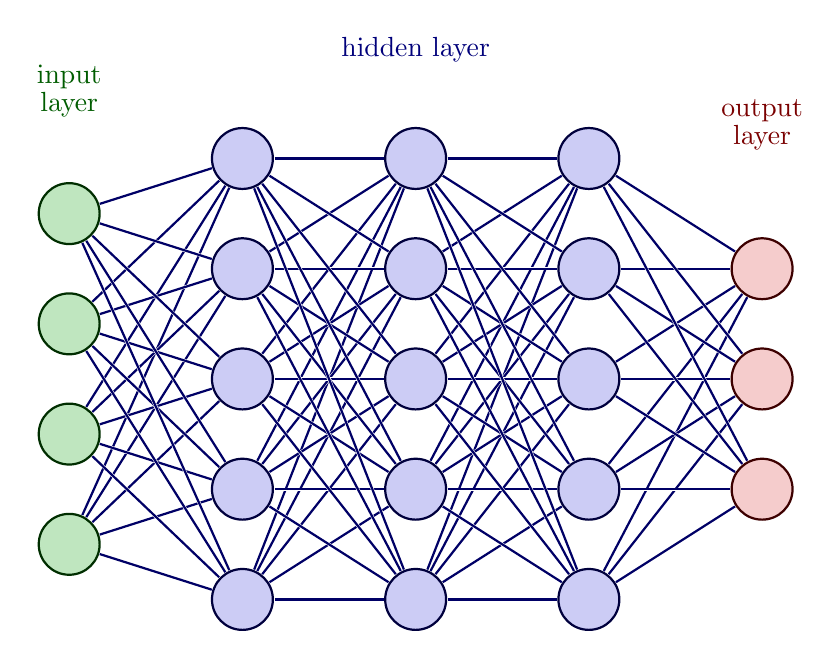
\begin{tikzpicture}[scale=1, x=2.2cm,y=1.4cm ]
  \message{^^JNeural network without text}
  \readlist\Nnod{4,5,5,5,3} % array of number of nodes per layer
  
  \message{^^J  Layer}
  \foreachitem \N \in \Nnod{ % loop over layers
    \def\lay{\Ncnt} % alias of index of current layer
    \pgfmathsetmacro\prev{int(\Ncnt-1)} % number of previous layer
    \message{\lay,}
    \foreach \i [evaluate={\y=\N/2-\i; \x=\lay; \n=\nstyle;}] in {1,...,\N}{ % loop over nodes
      
      % NODES
      \node[node \n] (N\lay-\i) at (\x,\y) {};
      
      % CONNECTIONS
      \ifnum\lay>1 % connect to previous layer
        \foreach \j in {1,...,\Nnod[\prev]}{ % loop over nodes in previous layer
          \draw[connect,white,line width=1.2] (N\prev-\j) -- (N\lay-\i);
          \draw[connect] (N\prev-\j) -- (N\lay-\i);
          %\draw[connect] (N\prev-\j.0) -- (N\lay-\i.180); % connect to left
        }
      \fi % else: nothing to connect first layer
      
    }
  }
  
  % LABELS
  \node[above=0.5,align=center,mygreen!60!black] at (N1-1.90) {input\\[-0.2em]layer};
  \node[above=0.5,align=center,myblue!60!black] at (N3-1.90) {hidden layer};
  \node[above=0.7,align=center,myred!60!black] at (N\Nnodlen-1.90) {output\\[-0.2em]layer};
  
\end{tikzpicture}
% \captionof{figure}{Simple Neural Network \cite{mit_neural_networks}} 
\caption{Feed Forward Neural Network \cite{tikz_neural_networks}}
\label{fig:ffnn}
\end{figure}

\begin{figure}
    \centering
    \includegraphics[width=0.5\textwidth]{neural_networks_brain.png}
    \caption{Brain Neural Network Simulation}
    \label{fig:simulation_brain}
\end{figure}


\bigskip

Both pictures show neurons or nodes propagating information.

The central component of a neural network is the artificial neural neuron (See Figure \ref{fig:ANN}), whose inspiration in the human brain comes from the nerve cells (See Figure \ref{fig:HN}).

\begin{figure}
    \centering
     \includegraphics[scale=0.4]{neural_network_mit.png}
    \caption{Artificial Neural Neuron \cite{mit_neural_networks}}
    \label{fig:ANN}
\end{figure}

\begin{figure}
    \centering
    % Second image (your external PNG)
    \includegraphics[scale=0.25]{Neuron.png}
    \caption{Human Neuron \cite{seer_neurons}}
    \label{fig:HN}
\end{figure}
The neuron is the processing unit in the architecture. One of the earliest models of such a unit is the perceptron, introduced by Frank Rosenblatt \cite{block1962perceptron}, which performs a weighted sum of inputs. It is a linear classifier for binary classification that computes the sum:

\begin{equation}
z = \sum w_i x_i + b
\end{equation}

where \( w_i \) are the weights, \( x_i \) are the inputs, and \( b \) is the bias term, which prevents the decision boundary from being constrained to pass through the origin. The output is then determined by the function:

\begin{equation}
f(z) =
\begin{cases} 
1, & \text{if } z \geq 0 \\
0, & \text{if } z < 0
\end{cases}
\end{equation}


The neurons are arranged in layers. Each layer uses the previous layer's outputs for its calculations and then forwards its outputs to the next layer.

Neurons are arranged in layers. Each layer uses the previous layer's outputs for its calculations and then forwards its outputs to the next layer.  For a given layer \( l \), the computation follows:

\begin{equation}
    z^{(l)} = W^{(l)} a^{(l-1)} + b^{(l)}
\end{equation}

\begin{equation}
    a^{(l)} = \sigma(z^{(l)})
\end{equation}

where \( W^{(l)} \) is the weight matrix, \( a^{(l-1)} \) represents the outputs (activations) from the previous layer, \( b^{(l)} \) is the bias vector, and \( \sigma(\cdot) \) is the activation function. 

There are typically three kinds of layers:

\textbf{Input Layer}

The input layer is a symbolic name since it refers to the input data points, with each node in the layer usually representing a feature of the data points. There is just one input layer.

\textbf{Hidden Layer} 

This is where the bulk of operations take place. They usually compose the majority of the layers.

\textbf{Output Layer}

Aggregates the inputs of the last hidden layer making sense of the data to get an output, which should be interpretable as a result of the specific task (regression, classification).


For complex tasks usually many hidden layers are required in neural networks, which define and give the name to the field of deep learning.

\subsubsection{Training}

The following explanation refers specifically to supervised training.

Training a model can be viewed as a minimization problem where the goal is to minimize this loss function over time. This process of minimization is what enables the model to improve its predictions.

There are typically two stages in a training loop: forward pass and backpropagation.

\textbf{Forward Pass}

Defines the process of a set of inputs, called batches in the context of training, going from the input layer to the output layer, which is essentially the prediction process.

\textbf{Backpropagation}

An algorithm to update weights in all layers using gradient descent following the chain rule in order to propagate from the last layer to the first hidden layer.
    % \todo{Lastly introduce natural language processing as one of the fields in which neural networks and deep learning are largely used}

\subsection{Natural Language Processing}

As the name implies, this field involves analyzing natural language (human language) and sometimes predicting from it. It is largely viewed as a subfield of machine learning since the most common approach used in modern Natural Language Processing (NLP) is deep learning.

\subsubsection{Embeddings}
Since the operations involved in training and prediction of neural networks are only defined with numerical data, a two-way representation between natural language and tensors of numbers is needed. The numerical representation is usually called embedding.

The first step to process input text is breaking it up into tokens, which in modern approaches are usually sub-words, averaging about 4 characters in length in the English language \cite{OpenAITokens}.

These tokens are then usually mapped to IDs through the vocabulary, which is a look-up table mapping text tokens to numeric IDs.

Finally, additional contextual information is embedded into the IDS during training of most modern models in NLP. They are updated based on surrounding tokens and relative position. For example the token "how" could have different embeddings in the sentences "How are you?" and "That is how you do it".

\subsection{Large Language Models}

Refer to deep learning models focusing on NLP, mainly on text. They have a large number of parameters, which gives them their name and are currently the state-of-the-art solution in the field of Natural Language Processing. They are the current answer to the high complexity posed by natural language, such as cultural references, syntax, semantics, and nuance.

The current most used architecture is called the Transformer Architecture and it aims to tackle the lack of parallelization possible in the previous models, sequential in essence \cite{vaswani2017attention}. It reduces training time significantly, in a task like translation between languages, from several days \cite{bahdanau2014neural} to as little as twelve hours.


\subsection{Transformer Architecture}


The main new breakthrough coming with the transformer architecture is the ability to process tokens in parallel while also keeping the dependencies of the ones far apart in the text input. This provides both a significant speed up in training as well as an increase in performance in certain tasks such as machine translation from English to German \cite{vaswani2017attention}.

\subsection{Transfer Learning}

Refers to leveraging training in one task to train a machine learning model in another, usually related task. \cite{torrey2010transfer}. 

A special kind of transfer learning, called cross-lingual transfer, revolves around leveraging training in one language to improve the results of training in another language \cite{cross_lingual_transfer}.

\subsection{Continual Pre-training of Large Language Models}
Refers to the addition of new data as knowledge base to an already trained large language model without merging the old dataset and the new one to start the training from scratch \cite{gupta2023continual}.

It consists mainly of the careful selection of a learning rate to minimize the loss on new data while maintaining the loss on the original data. This is a key factor in the process since the distribution shift that further training introduces can lead to a decrease in performance in previous (original) data. Research indicates that the right parameters might make continual pre-training better performing than training from scratch on the whole data \cite{gupta2023continual}.


\subsection{Semantic Web}

An initiative to make web content machine-readable by standardizing it \cite{pellegrini2006semantic}.

Resource Description Framework (RDF) is one of the most popular frameworks for standardizing and representing web content. It was first introduced and encouraged by the World Wide Web Consortium (Organization developing the standards of the Web) in 1999 \cite{dataeuropa_rdf_sparql}, proposing a graph structure linking web contents making the relationships between contents machine-readable, with SPARQL being the standard query language for this format.





\section{Research Background}\label{section::research_background}

\subsection{Transfer Learning}

Although the idea of leveraging the knowledge of previous training in new ones was already introduced in neural networks in the 1970s \cite{bozinovski2020reminder}, the first successful case of using it in NLP in the context of pre-trained LLMs was in 2015 \cite{HAN2021225}.

With the introduction of GPT-3, it was shown to be possible to train an LLM on a "general-purpose text generation" downstream task, typically called fine-tuning \cite{WANG202351}. Since then, transformer-based LLMs have been gaining in popularity and in performance because of the flexibility and relatively small set of data required to effectively train for the downstream tasks.

Different methods have been developed to cater to small datasets and low hardware resources, by lowering the tunable parameters and the model's precision \cite{parthasarathy2024ultimate}.
\subsection{Cross-Lingual Transfer}

% general cross lingual transfer

Before the rise in popularity of llms, Cross-lingual transfer had been continually studied within neural networks in the context of NLP for specific tasks, such as part-of-speech tagging \cite{kim-etal-2017-cross}.

One of the most common challenges in NLP is improving performance in low-resource languages (languages with small amounts of training data). Usual approaches include tackling the model at the word embedding level leveraging high resource languages, translating training data \cite{schuster2018cross} and changing the model architecture \cite{pfeiffer2020mad}.

With the rise of LLms, cross-lingual transfer kept being studied within its context, focusing initially on specific tasks such as part-of-speech tagging with zero-shot learning (no training samples) \cite{adelani2024comparing}.

Architectural approaches such as adding adapter layers (trainable layers) to transformer-based models and training them are one of the popular techniques to improve zero-shot cross-lingual transfer \cite{10.1145/3581783.3611992} along with previously researched word embedding approaches that increase the similarity of word embeddings between languages \cite{efimov2023impact}.

Factors surrounding the degree of cross-lingual transfer developed by LLMs with multilingual pre-training have been studied before \cite{fujinuma2022match}, and a surge in interest in it has been showing recently in current research \cite{wang2024probing}.


\subsection{Text-to-SPARQL}

There are in general three approaches used for LLMs to extract knowledge from data in RDF format to answer questions in natural language \cite{avila2024experiments}.

The first one is to provide the dataset to the LLM along with the question, so that it answers the questions directly \cite{avila2024experiments}.

The second approach is to translate the question from natural language to a SPARQL query that then gets executed in the corresponding engine. This approach often relies on prompt engineering \cite{zahera2024generating} (structuring of prompt to leverage Llm capabilities \cite{aws_prompt_engineering}).

The third approach is a combination of the first two. It involves getting the right parts of the data to feed them to the LLM to generate the SPARQL query with prompt engineering \cite{emonet2024llm}.

\section{Contribution}\label{section::contribution}

\section{Methodology}\label{section::methodology}

\subsection{Data Collection}
\todo{Which datasets did we draw from?}

Data is drawn from all of the QALD (Question Answering over Linked Data) challenges until now, from the first edition to the tenth edition. The goal of this challenge is for teams to compete to extract information from knowledge graphs in the most accurate way \cite{LOPEZ20133}, aligning well with the first goal of creating a multilingual dataset for text-to-SPARQL generation.

The data from the QALD challenges were combined with most of the different datasets gathered by Jian et al. \cite{jiang2022knowledge} from different challenges regarding question-answering over knowledge graphs. Specifically, the challenges drawn upon are those from Talmor et al. \cite{Talmor2018TheWA}, Cui et al. \cite{2021arXiv210803509C}, Gu et al. \cite{gu2021beyond}, Su et al. \cite{su-etal-2016-generating, s}, Trivedi et al. \cite{trivedi2017lc}, Dubey et al. \cite{dubey2017lc2}, Kaffee et al. \cite{DBLP:conf/kcap/KaffeeESV19}, Korablinov et al. \cite{2020arXiv200510659K}, Rybin et al. \cite{rybin2021rubq} and Yih et al. \cite{yih-etal-2016-value}. The datasets in consideration meet the basic requirement of having the following properties available or easily inferable for each question: question in natural language, SPARQL query, language and knowledge graph referenced.

For the QALD datasets, a script was made to scrape the main QALD repository (https://github.com/ag-sc/QALD/tree/master), which has the QALD challenges from 1 to 9, with the data of all challenges, to check that the schema meets the basic requirements for the task, and merge them into the standardized schema with the following columns: text\_query, language, sparql\_query and knowledge\_graphs. Since the datasets in the rest of the challenges, with the exception of QALD 10, had much more varied forms, each dataset had to be manually examined to check the schema and a custom script was made to extract all of its partitions, adapt the schema, and combine with the previously merged dataset.

\subsection{Data Analysis}

\todo{Numbers. How big were the QALD datasets in total, how big were the others, were some of them particularly big?}

The QALD datasets sum up to about 16000 data points, while the rest make up around 620000. One dataset stands out because of its size, the Multilingual Compositional Wikidata Questions dataset by Cui et al. \cite{2021arXiv210803509C} with around 100000 questions in each of the following languages: English, Hebrew, Kannada and Chinese. It is worth pointing out that the non-English questions were translated from English using Google Translation.

Regarding the data quality, the QALD 10 dataset stands out for being a multilingual dataset curated by native speakers, It provides 806 questions, each one in Chinese (Mandarin), English, German and Russian with the corresponding SPARQL query for the knowledge graph Wikidata.

\todo{common small errors and where do they come from}
\iffalse
There were some small orthographic errors as for example the word character written as "charcter" in the following question: "In the film that has a charcter named Rev. Jackson P. Sayer, who played Michael Myers?" from the dataset Complex Web Questions by Talmor et al. 
\fi

\iffalse
Some of the questions are incomplete like the question in french "Quel est le" in the QALD 5 dataset which would be translated in English as "What is the"
\fi
\todo{talk about the length of the queries and its relationship with the quality and which dataset had the higher quality}

\iffalse
In regards of data quality, the QALD 10 dataset stands out for being a multilingual dataset curated by native speakers. It provides 806 questions, each question in Chinese (Mandarin), English, German and Russian with the corresponding SPARQL query on the knowledge graph Wikidata. 
\fi


\todo{How does the final dataset look like: size, how many languages, which knowledge graphs, how is the length of the text queries? was there some relationship between the data quality and the length of text queries?}

\section{Experimental Setup}\label{section::experimental_setup}

\subsection{Data Processing}

\subsection{Training}



\section{Results}\label{section::results}


\subsection{Mistral}


\subsection{Occiglot}


\section{Discussion}\label{section::discussion}

\subsection{Comparison}

\subsection{Interpretation}

\input{chapters/09_conclusion}


%%%%%%%%%%%%%%%%%%%%%%%%%%%%%%%%%%%_BIBLIOGRAPHY_%%%%%%%%%%%%%%%%%%%%%%%%%%%%%%%%%%%
% create your bibliography based on your files in library/...
% remember to edit \addbibresource in the TEMPLATE_PACKAGSES area above!
\newpage
\pagenumbering{roman} % start roman page numbers from here (optional)
% \bibliographystyle{abbrv}
% \bibliography{library/citations.bib}
\printbibliography
%%%%%%%%%%%%%%%%%%%%%%%%%%%%%%%%%%%%%_APPENDIX_%%%%%%%%%%%%%%%%%%%%%%%%%%%%%%%%%%%%
\section*{Appendix} \label{Appendix}
\addcontentsline{toc}{section}{Appendix}    % adds entry to table of contents
\declarationofintegrity{\today}
%\input{chapters/xxx}                       % add in case you have additional images/tables
\end{document}
%%%%%%%%%%%%%%%%%%%%%%%%%%%%%%%%%%%%%%%%%%%%%%%%%%%%%%%%%%%%%%%%%%%%%%%%%%%%%%%%%%%%
